\begin{frame}{Limitations of SLP}
	\begin{itemize}
		\item What are the limitations of SLP?
		\item Can we learn all functions with SLP?
	\end{itemize}
	\begin{figure}[H]
		\centering
		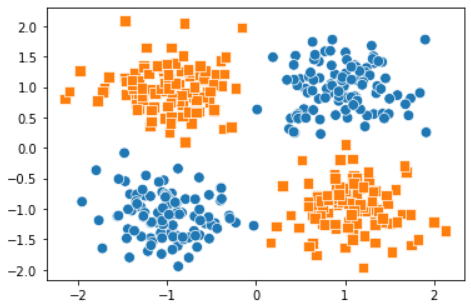
\includegraphics[width=0.6\textwidth]{Figs/xor.png}
		\caption{The XOR function is not linear separable.}
	\end{figure}
\end{frame}

\begin{frame}{Limitations of SLP}
	\begin{itemize}
		\item As we saw in the XOR case, nonlinear separable functions can not be learned by SPLs.
	\end{itemize}
	\begin{figure}[H]
		\centering
		\begin{subfigure}[b]{0.4\textwidth}
			\centering
			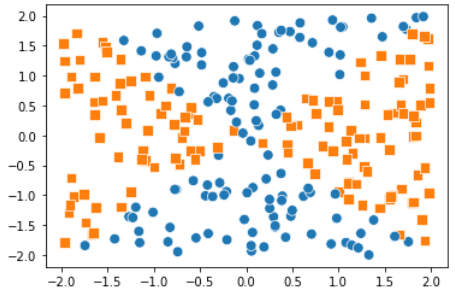
\includegraphics[width=\textwidth]{Figs/non-linear1.png}
		\end{subfigure}
		\hspace*{1.5em}
		\begin{subfigure}[b]{0.4\textwidth}
			\centering
			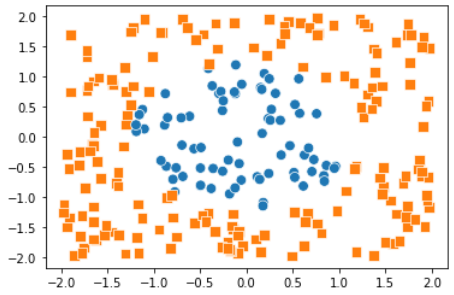
\includegraphics[width=\textwidth]{Figs/non-linear2.png}
		\end{subfigure}
		\caption{Examples of nonlinear separable functions.}
	\end{figure}    
	\begin{itemize}
		\item How to solve this?
	\end{itemize}
\end{frame}

\begin{frame}{Limitations of SLP}
	\begin{itemize}
		\item What if we knew some feature space which our data is linear separable in?!
	\end{itemize}
	\begin{figure}[H]
		\centering
		\begin{subfigure}[b]{0.35\textwidth}
			\centering
			$(x, y)$
			$\vcenter{\hbox{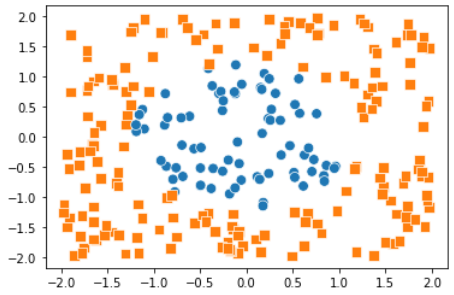
\includegraphics[width=\textwidth]{Figs/non-linear2.png}}}$
		\end{subfigure}
		$\quad\Longrightarrow\quad$
		\begin{subfigure}[b]{0.35\textwidth}
			\centering
			$(r, \theta)$
			$\vcenter{\hbox{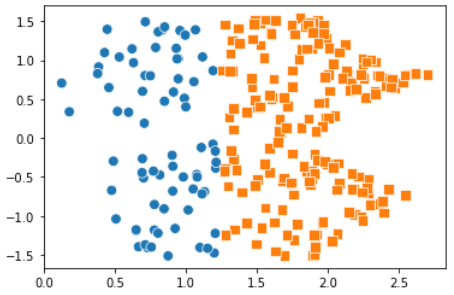
\includegraphics[width=\textwidth]{Figs/circ-linear.png}}}$
		\end{subfigure}
		\caption{Data is linear separable after transformation.}
	\end{figure}
\end{frame}

\begin{frame}{Multi-Layer Perceptron}
	\begin{itemize}
		\item So if we know some $f_1, \cdots, f_4$ we can use SLP to solve problem.
	\end{itemize}
	\begin{figure}[H]
		\centering
		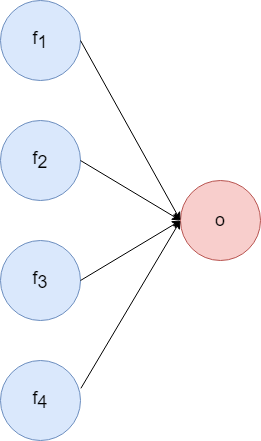
\includegraphics[height=0.45\textheight]{Figs/feature_space.png}
		\caption{Using feature space $f$ to solve problem.}
	\end{figure}
	\begin{itemize}
		\item How to learn this $f_i$s? Use SLP!
	\end{itemize}
\end{frame}

\begin{frame}{Multi-Layer Perceptron}
	\begin{itemize}
		\item We can use inputs ($x_i$) to learn features ($f_i$)
	\end{itemize}
	\begin{figure}[H]
		\centering
		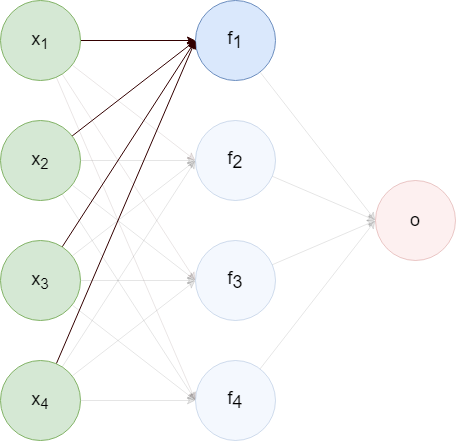
\includegraphics[height=0.45\textheight]{Figs/learn_features.png}
		\caption{Using inputs to learn features.}
	\end{figure}
	\begin{itemize}
		\item What if $f_i$s are not sufficient? We can add more layers!
	\end{itemize}
\end{frame}

\begin{frame}{Multi-Layer Perceptron}
	\begin{itemize}
		\item Adding more layers we will have a bigger network.
	\end{itemize}
	\begin{figure}[H]
		\centering
		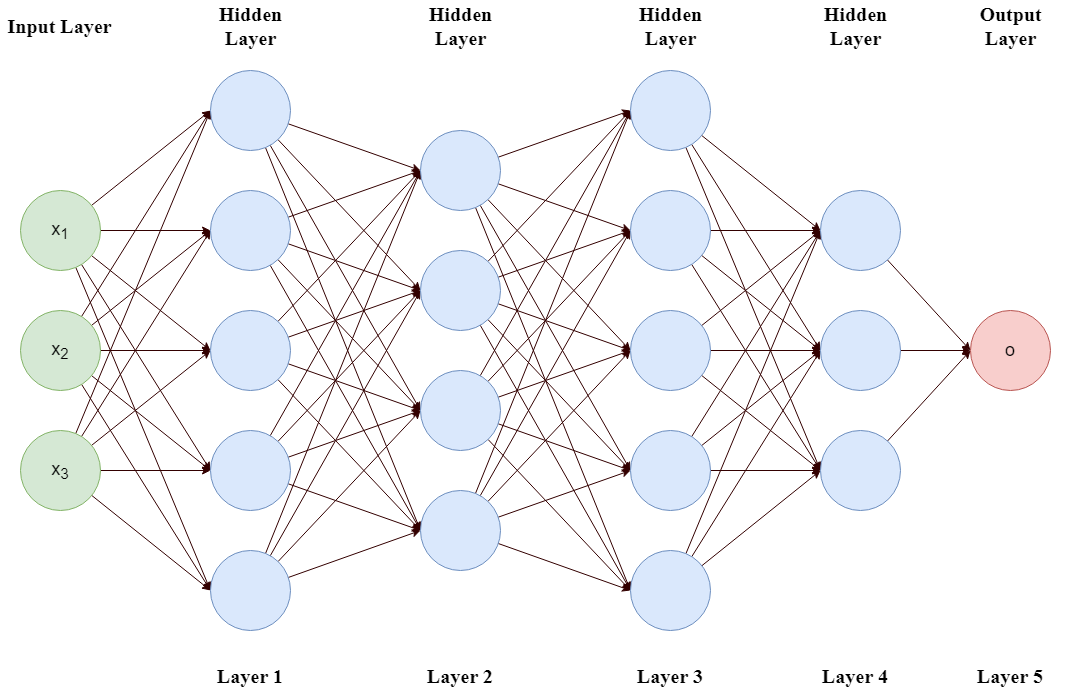
\includegraphics[width=0.8\textwidth]{Figs/5layer_mlp.png}
		\caption{A 5 layer MLP.}
	\end{figure}
\end{frame}


\begin{frame}{Architecture of MLPs}
	\begin{itemize}
		\item Important questions:
		\begin{itemize}
			\item How many hidden layer should we have?
			\item In each hidden layer, how many neuron should we have?
		\end{itemize}
	\end{itemize}
	\begin{figure}[H]
		\centering
		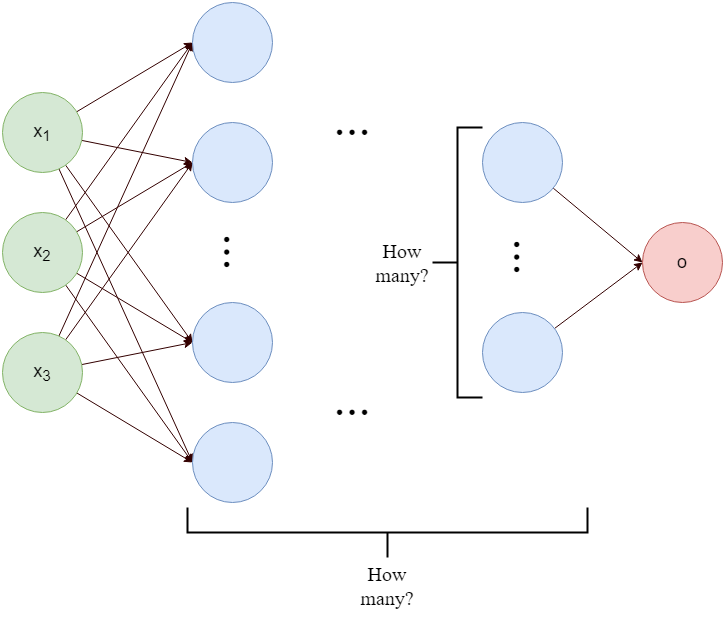
\includegraphics[height=0.6\textheight]{Figs/how_many_layer.png}
		\caption{How many layers and neurons should we have?}
	\end{figure}
\end{frame}


% \begin{frame}{Architecture of MLPs}
	%     \begin{itemize}
		%         \item In theory:
		%         \begin{itemize}
			%             \item You will have unlimited resources
			%             \item (1 hidden layer, $\infty$ neurons) will be sufficient to learn any function 
			%         \end{itemize}
		%     \end{itemize}
	%     \begin{figure}[H]
		%         \centering
		%         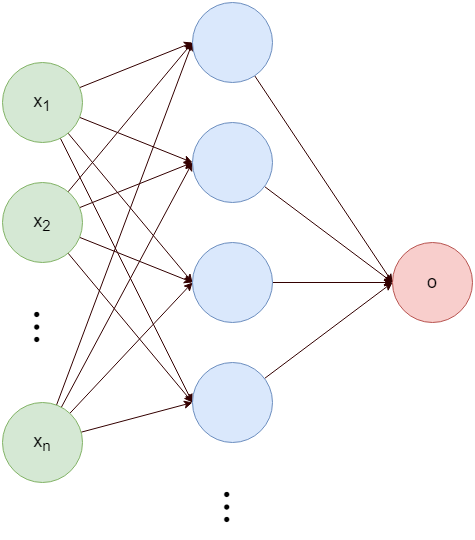
\includegraphics[height=0.5\textheight]{Figs/inf_neuron.png}
		%         \caption{1 hidden layer and $\infty$ neuron.}
		%     \end{figure}
	% \end{frame}


\begin{frame}{Architecture of MLPs}
	\begin{itemize}
		\item In practice:
		\begin{itemize}
			\item You have limited resources
			\item There is no universal rule to choose this hyperparameters
			\item Need to experiment for different number of layers and neurons in each layer
		\end{itemize}
	\end{itemize}
	\begin{figure}[H]
		\centering
		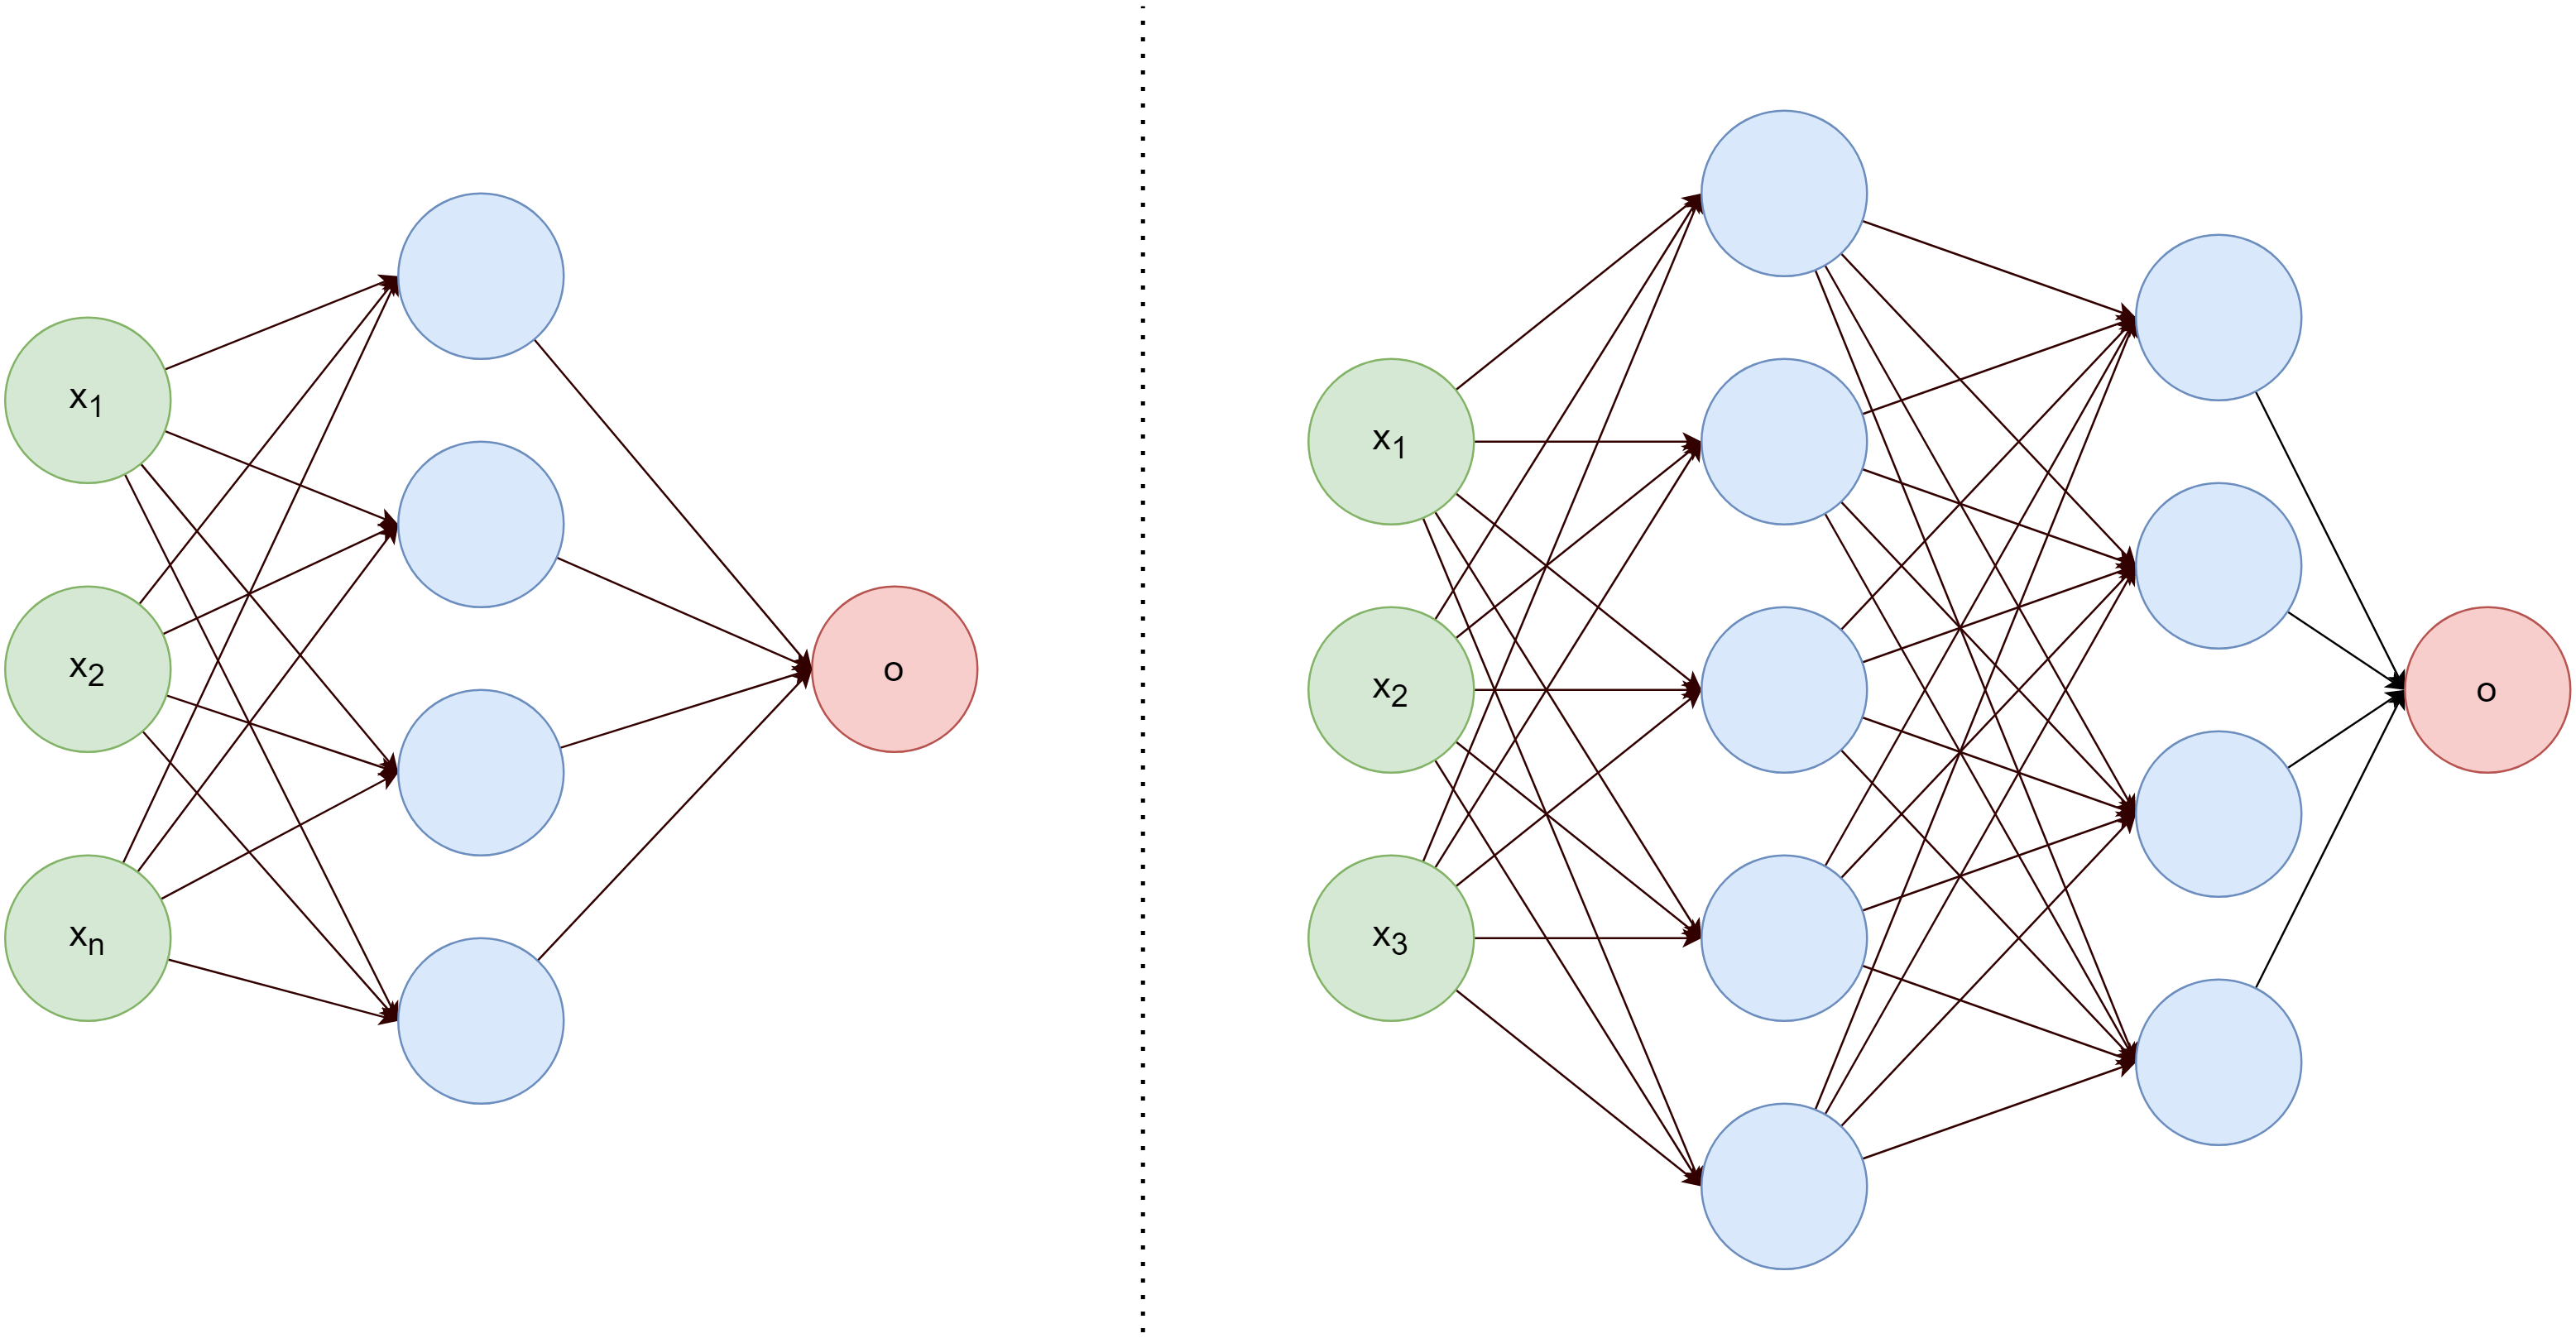
\includegraphics[width=0.6\textwidth]{Figs/experiment_arch.png}
		\caption{Experiment for different architecture and choose the best model.}
	\end{figure}
\end{frame}

\begin{frame}{Activation Function of Hidden Layers}
	\begin{itemize}
		\item One can use any activation function for each hidden units
		\item Usually people use the same activation function for all neurons in one layer
		\item The important point is to use \tc{keywords}{nonlinear} activation functions
	\end{itemize}
	\begin{figure}[H]
		\centering
		\begin{subfigure}[b]{0.55\textwidth}
			\centering
			$\vcenter{\hbox{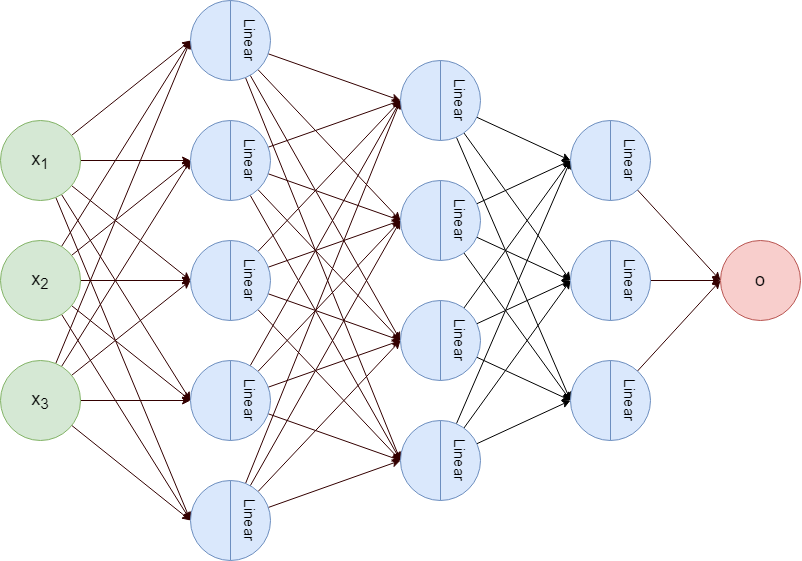
\includegraphics[width=\textwidth]{Figs/linear_neurons.png}}}$
		\end{subfigure}
		$\quad\equiv\quad$
		\begin{subfigure}[b]{0.15\textwidth}
			\centering
			$\vcenter{\hbox{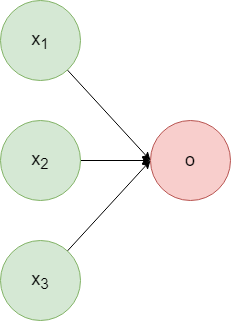
\includegraphics[width=\textwidth]{Figs/simple_slp.png}}}$
		\end{subfigure}
		\caption{MLP with linear activation functions is equivalent to simple SLP.}
	\end{figure}
\end{frame}

\begin{frame}{XOR problem}
	\begin{itemize}
		\item Now let's solve XOR problem with MLPs.
		\item We have two binary inputs, build an MLP to calculate their \textbf{XOR}.
		\medskip
		\medskip
		\item First let's build logical \textbf{AND} and \textbf{OR} functions.
	\end{itemize}
	\begin{figure}[H]
		\centering
		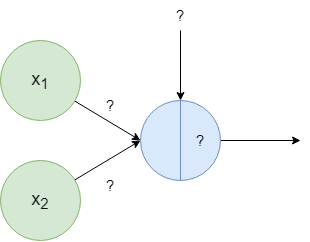
\includegraphics[width=0.35\textwidth]{Figs/solve_and_or_gate.png}
		\caption{We need to find weights, biases and activation function.}
	\end{figure}
\end{frame}

\begin{frame}{XOR problem}
	\begin{figure}
		\centering
		\begin{subfigure}[b]{0.25\textwidth}
			\centering
			$\vcenter{\hbox{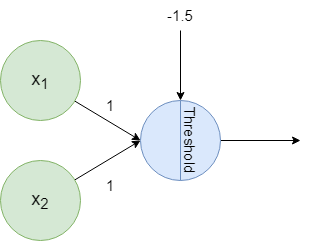
\includegraphics[width=\textwidth]{Figs/and_gate.png}}}$
			\caption{$x_1 \wedge x_2$}
		\end{subfigure}
		\hspace*{0.5em}
		\begin{subfigure}[b]{0.25\textwidth}
			\centering
			$\vcenter{\hbox{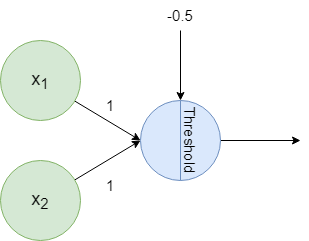
\includegraphics[width=\textwidth]{Figs/or_gate.png}}}$
			\caption{$x_1 \vee x_2$}
		\end{subfigure}
		\hspace*{0.5em}
		\begin{subfigure}[b]{0.25\textwidth}
			\centering
			$\vcenter{\hbox{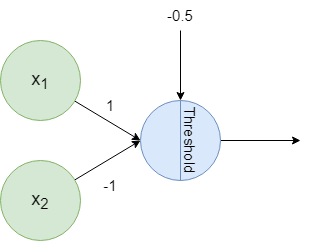
\includegraphics[width=\textwidth]{Figs/and_not_gate.png}}}$
			\caption{$x_1 \wedge \overline{x_2}$}
		\end{subfigure}
	\end{figure}
	\pause
	\begin{figure}[H]
		\centering
		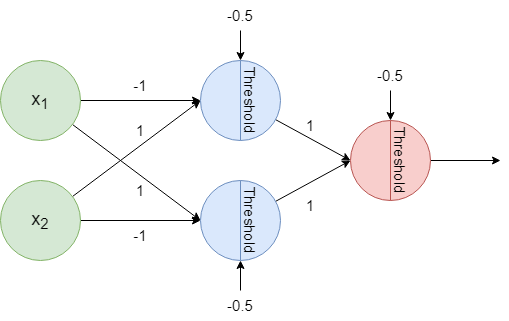
\includegraphics[height=0.35\textheight]{Figs/xor_gate.png}
		\caption{MLP for XOR function.}
	\end{figure}
\end{frame}


% \begin{frame}{Example of universality}
	%     \begin{itemize}
		%         \item ToDo
		%     \end{itemize}
	% \end{frame}


\begin{frame}{MLP notation}
	\begin{itemize}
		\item $a^{[l]}_i$: $i$-th neuron outpu in layer $l$
		\item $\bm{a}^{[l]}$: layer $l$ output in vector form
	\end{itemize}
	\begin{figure}[H]
		\centering
		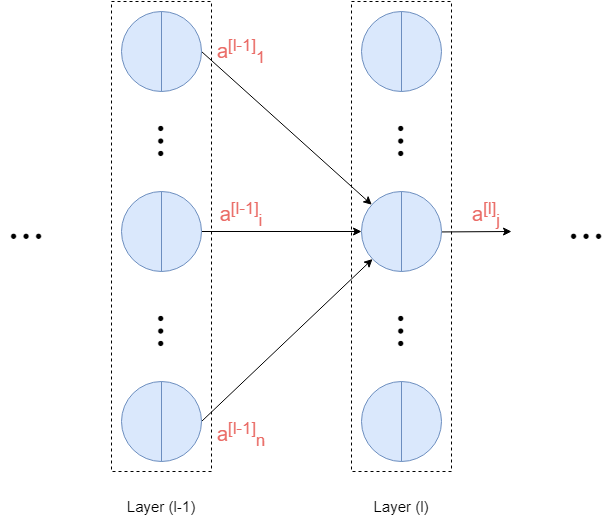
\includegraphics[width=0.5\textwidth]{Figs/notation1.png}
	\end{figure}
\end{frame}

\begin{frame}{MLP notation}
	\begin{itemize}
		\item $b^{[l]}_i$: $i$-th neuron biase in layer $l$
		\item $\bm{b}^{[l]}$: layer $l$ biases in vector form
	\end{itemize}
	\begin{figure}[H]
		\centering
		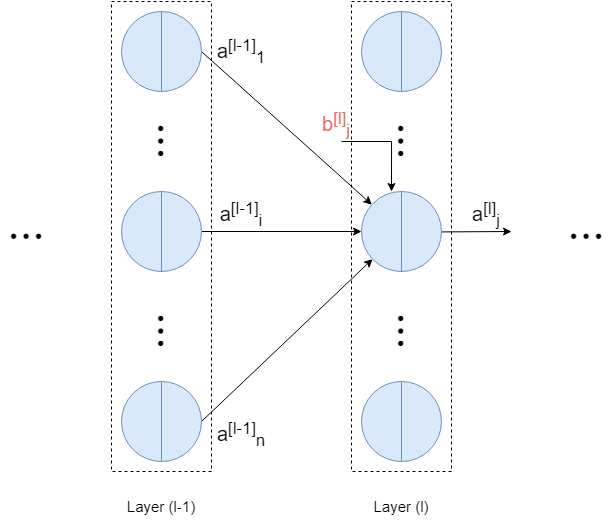
\includegraphics[width=0.5\textwidth]{Figs/notation1.2.png}
	\end{figure}
\end{frame}

\begin{frame}{MLP notation}
	\begin{itemize}
		\item $W^{[l]}_{ij}$: weight of the edge between $i$-th nuron in layer $l-1$ and $j$-th neuron in layer $l$ 
	\end{itemize}
	\begin{figure}[H]
		\centering
		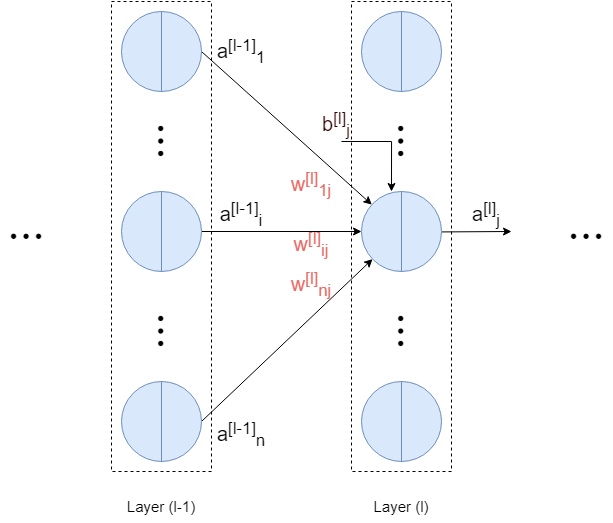
\includegraphics[width=0.5\textwidth]{Figs/notation2.png}
	\end{figure}
\end{frame}

\begin{frame}{MLP notation}
	\begin{itemize}
		\item $z^{[l]}_j$: $j$-th neuron input in layer $l$
		\item $z^{[l]}_j = b_j^{[l]} + \sum_{i=1}^n W^{[l]}_{ij}a^{[l-1]}_i$
	\end{itemize}
	\begin{figure}[H]
		\centering
		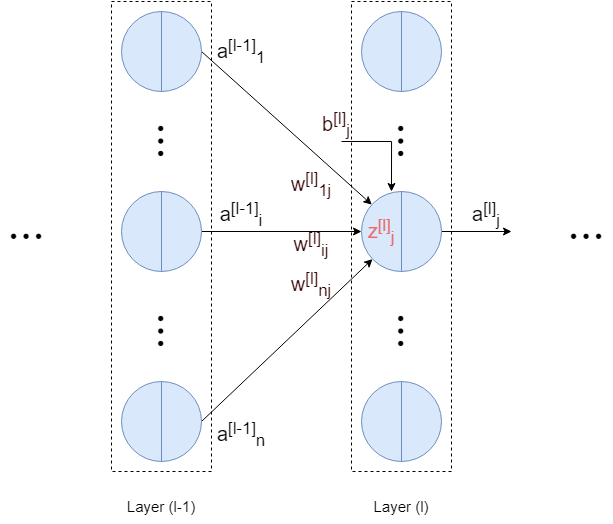
\includegraphics[width=0.5\textwidth]{Figs/notation3.png}
	\end{figure}
\end{frame}

\begin{frame}{MLP notation}
	\begin{itemize}
		\item $\bm{z}^{[l]}$: input of layer $l$ in vector form
		\item $\bm{z}^{[l]} = \bm{b}^{[l]} + (W^{[l]})^T \bm{a}^{[l-1]}$
	\end{itemize}
	\begin{figure}[H]
		\centering
		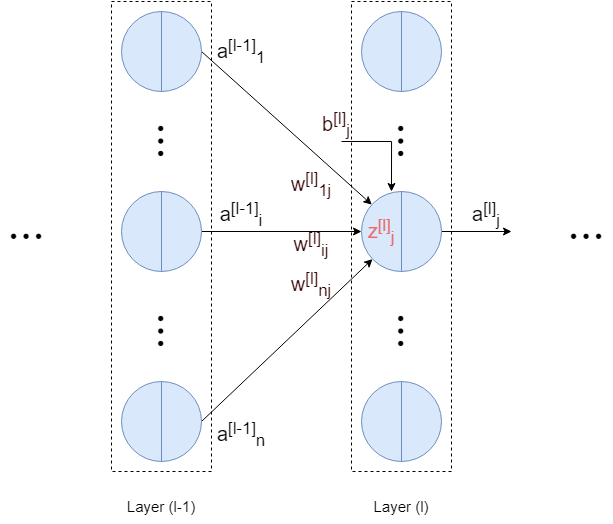
\includegraphics[width=0.5\textwidth]{Figs/notation3.png}
	\end{figure}
\end{frame}

\begin{frame}{MLP notation}
	\begin{itemize}
		\item $\sigma^{[l]}_j$: $j$-th neuron activation function in layer $l$
	\end{itemize}
	\begin{figure}[H]
		\centering
		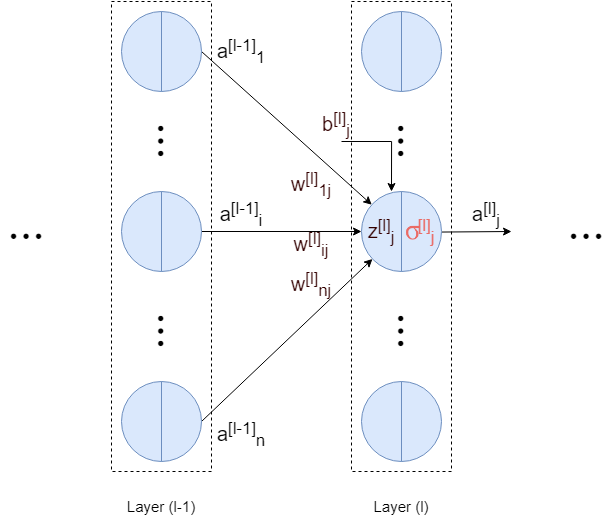
\includegraphics[width=0.5\textwidth]{Figs/notation4.png}
	\end{figure}
\end{frame}

\begin{frame}{MLP notation}
	\begin{itemize}
		\item If we assume all neurons in one layer have the same activation function then:
		\[
		\bm{a}^{[l]} = \sigma^{[l]}\left(\bm{b}^{[l]} +  (W^{[l]})^T\bm{a}^{[l-1]}\right)
		\]
	\end{itemize}
	\begin{figure}[H]
		\centering
		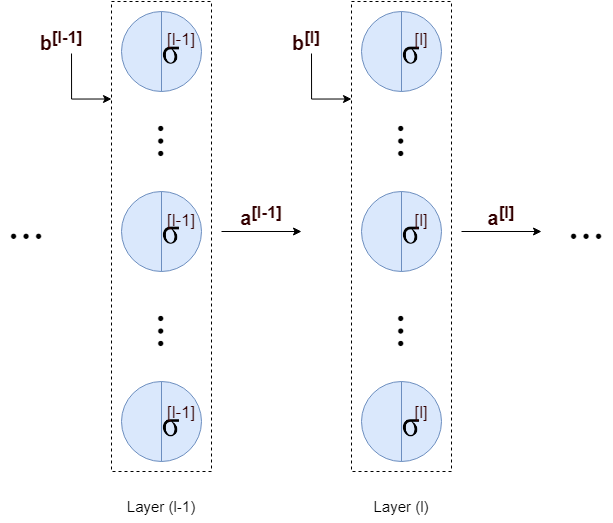
\includegraphics[width=0.5\textwidth]{Figs/notation5.png}
	\end{figure}
\end{frame}

\begin{frame}{MLP notation}
	\begin{itemize}
		\item So for a network with $L$ layer, and $\bm{x}$ as its input we will have:
	\end{itemize}
	\begin{figure}[H]
		\centering
		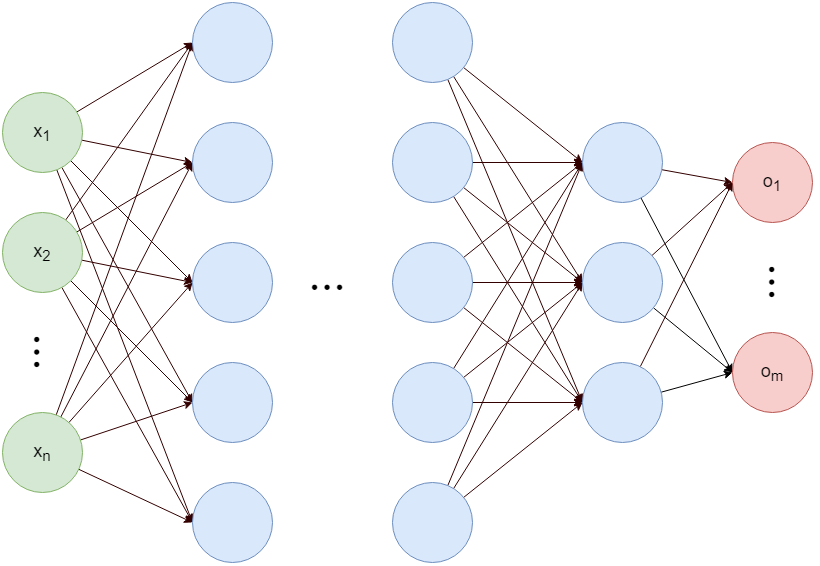
\includegraphics[width=0.6\textwidth]{Figs/notation6.png}
	\end{figure}
	% \[
	% \bm{o}=\bm{a}^{[L]}=\sigma^{[L]}\left((W^{[L]})^T\sigma^{[L-1]}\left((W^{[L-1]})^T\sigma^{[L-2]}\left(\cdots\sigma^{[1]}\left((W^{[1]})^T\bm{x}\right)\cdots \right)\right)\right)
	% \]
	\[
	\bm{o}=\bm{a}^{[L]}=\sigma^{[L]}\left(\bm{b}^{[L]} + (W^{[L]})^T\sigma^{[L-1]}\left(\cdots\sigma^{[1]}\left(\bm{b}^{[1]}+(W^{[1]})^T\bm{x}\right)\cdots \right)\right)
	\]
\end{frame}

\begin{frame}{Learning MLPs}
	\begin{itemize}
		\item Till here we have used networks with predefined weights and biases.
		\item How to learn these parameters?
		\medskip
		\medskip
		\medskip
		\item The idea is to use gradient descent
	\end{itemize}
	\begin{figure}
		\centering
		\begin{subfigure}[b]{0.3\textwidth}
			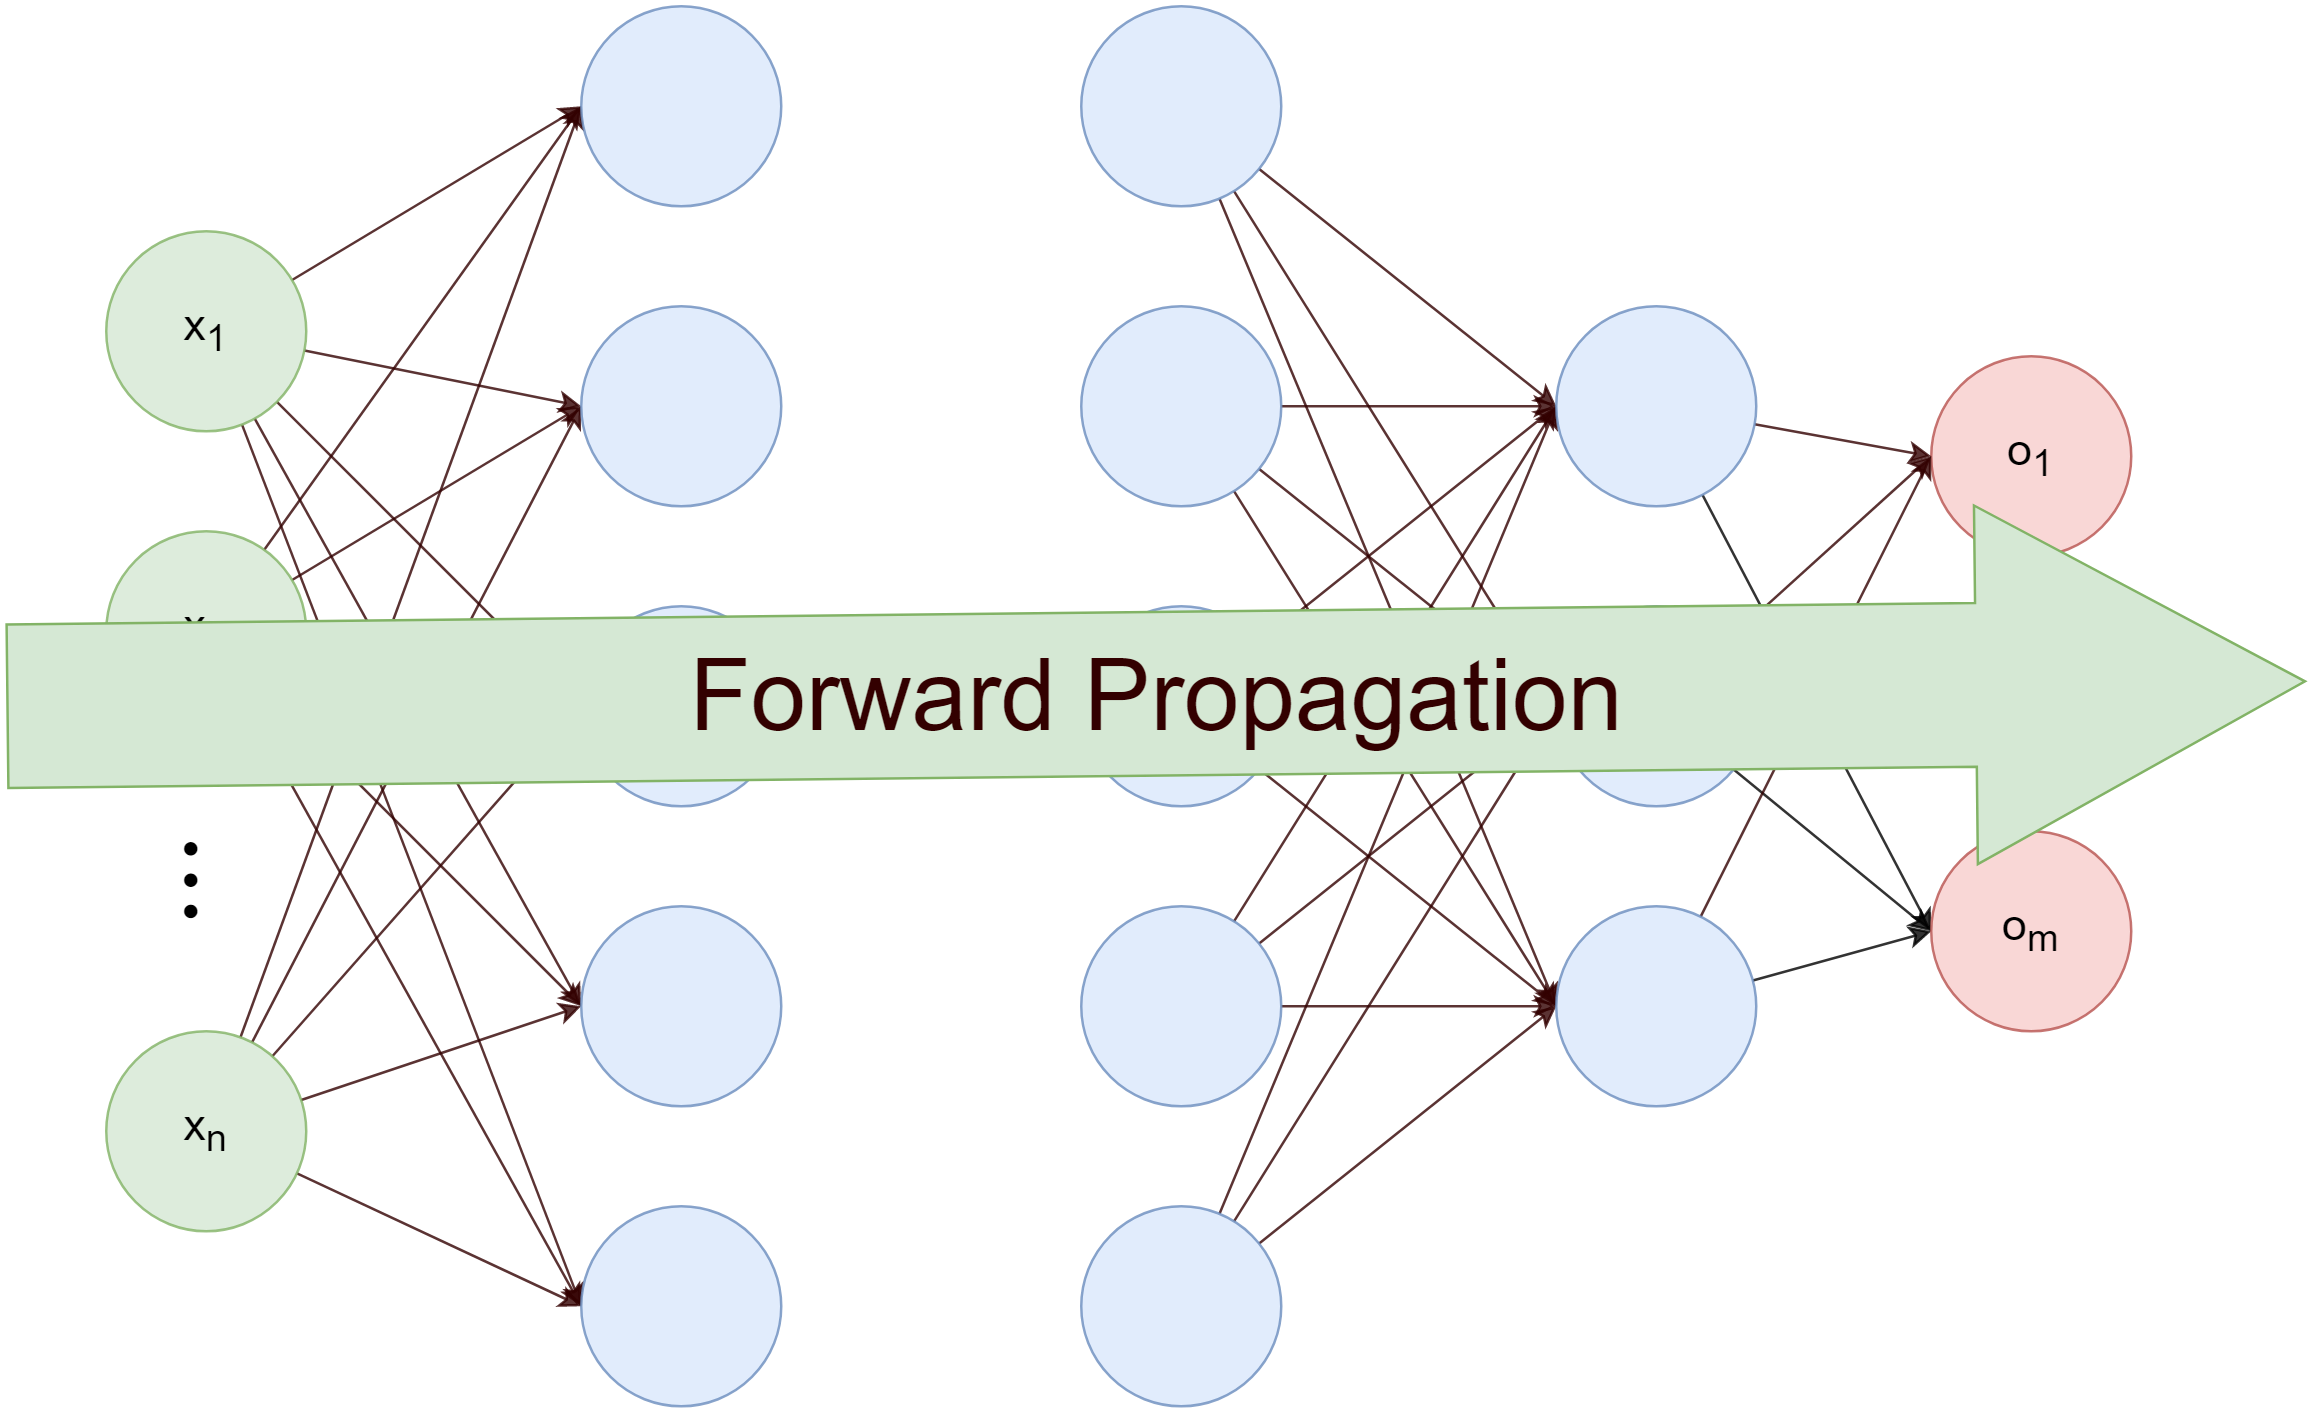
\includegraphics[width=\textwidth]{Figs/forward_propagation.png}
			\caption{Forward pass}
		\end{subfigure}
		\begin{subfigure}[b]{0.3\textwidth}
			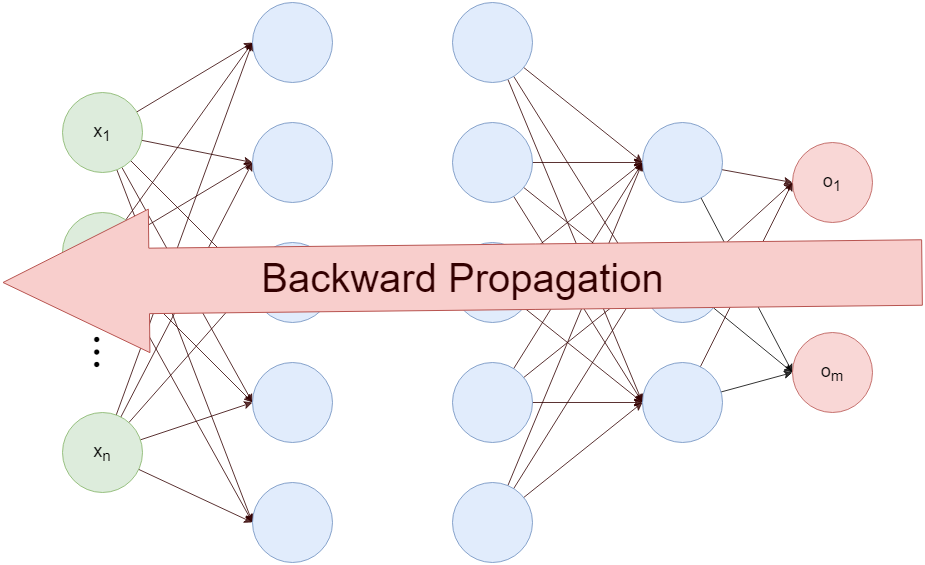
\includegraphics[width=\textwidth]{Figs/backward_propagation.png}
			\caption{Backward pass}
		\end{subfigure}
		\begin{subfigure}[b]{0.28\textwidth}
			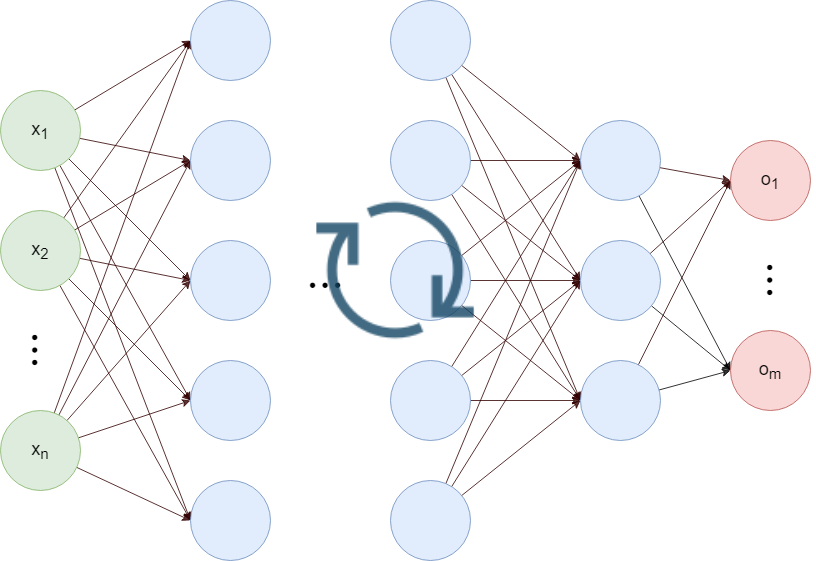
\includegraphics[width=\textwidth]{Figs/update_phase.png}
			\caption{Update parameters}
		\end{subfigure}
	\end{figure}
\end{frame}